\documentclass[xcolor=dvipsnames]{beamer}

\usetheme{Boadilla}

\newcommand{\bi}{\begin{itemize}}
\newcommand{\ei}{\end{itemize}}
\newcommand{\be}{\begin{enumerate}}
\newcommand{\ee}{\end{enumerate}}
\newcommand{\I}{\item}
\newcommand{\f}{\frame}
\newcommand{\ft}{\frametitle}


\begin{document}

\title{Pulls and Residuals}
\author[M.\ Ito]{Mark M.\ Ito}
\date{March 23, 2009}
\institute[JLab]{Jefferson Lab}

\f{
\ft{Starting Parameters: Two Options Explored}
\be
\I Guess
\bi
\I $p = \infty$
\I $\phi$ from connecting inner and outer hits
\I $\theta_{\rm CDC}$ from true shifted by $5^\circ$, $\theta_{\rm FDC}$ from connecting upstream and downstream hits
\I $r_0 = 0$
\I $z_0 = 65$~cm
\ei
\I True
\bi
\I Use parameters chosen by the MC
\I Swim from center of target
\ei
\ee
}

\f{
\ft{Residuals, Guess}
Residual RMS = 153 microns
$$
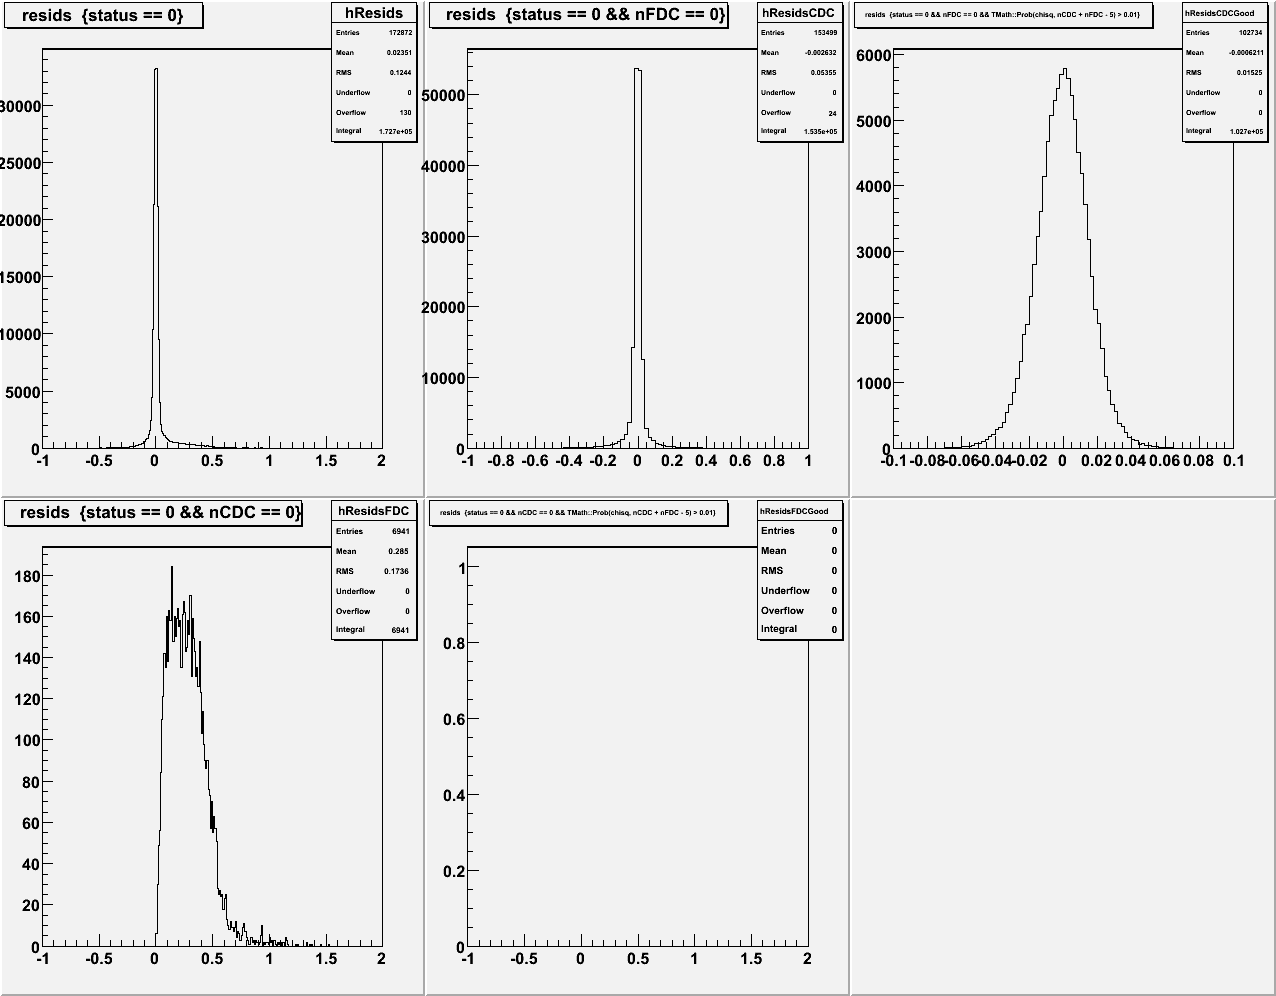
\includegraphics[height=3.0in]{resids_guess.png}
$$
}

\f{
\ft{Residuals, True}
ResidualRMS = 139 microns
$$
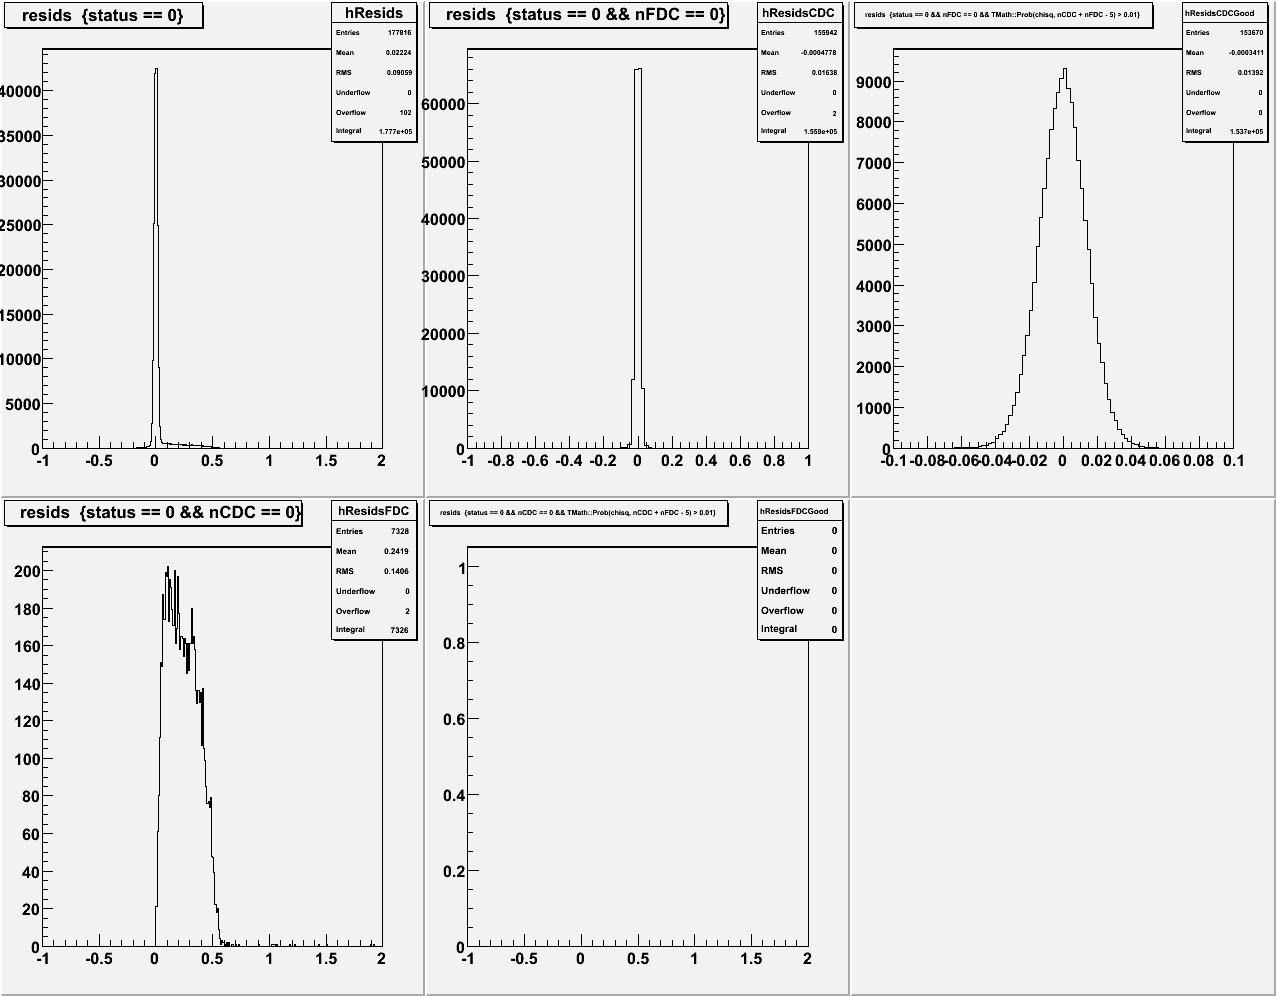
\includegraphics[height=3.0in]{resids_true.png}
$$
}

\f{
\ft{Chi-Squared, Guess}
$$
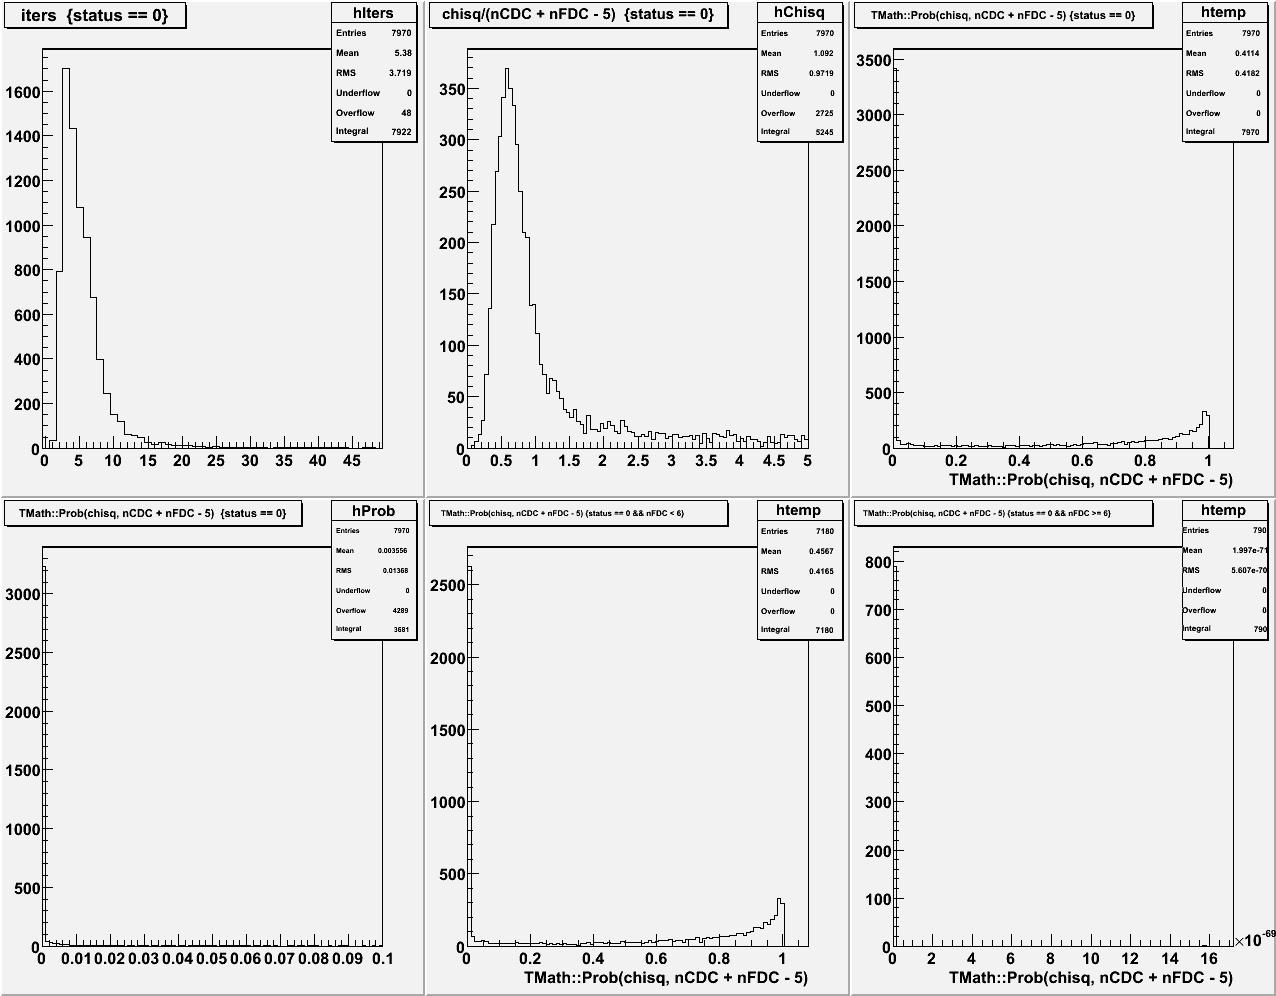
\includegraphics[height=3.0in]{chisq_guess.png}
$$
}

\f{
\ft{Chi-squared, True}
$$
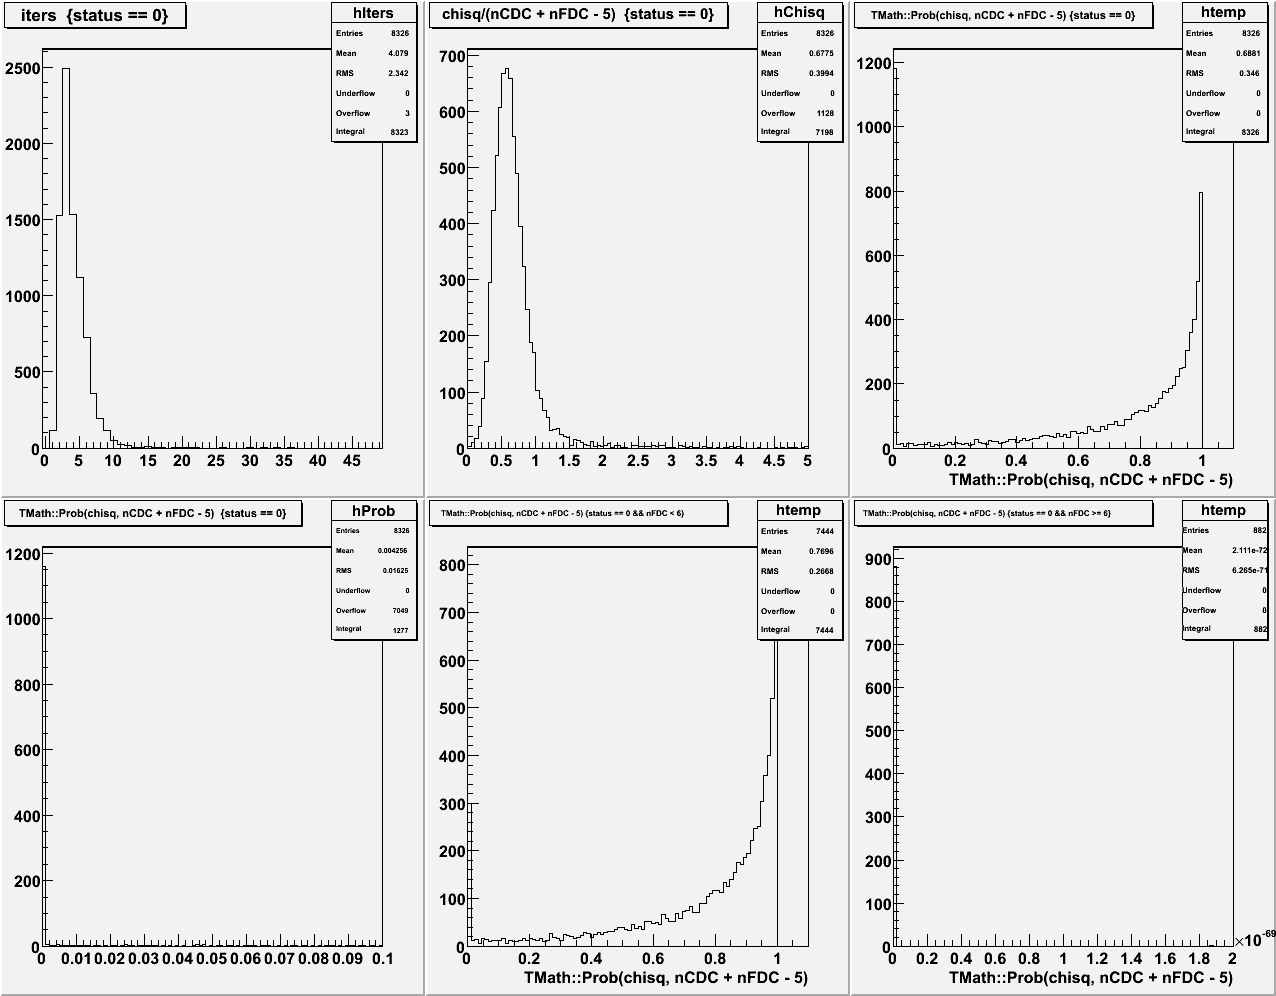
\includegraphics[height=3.0in]{chisq_true.png}
$$
}

\f{
\ft{Pulls, Guess}
$$
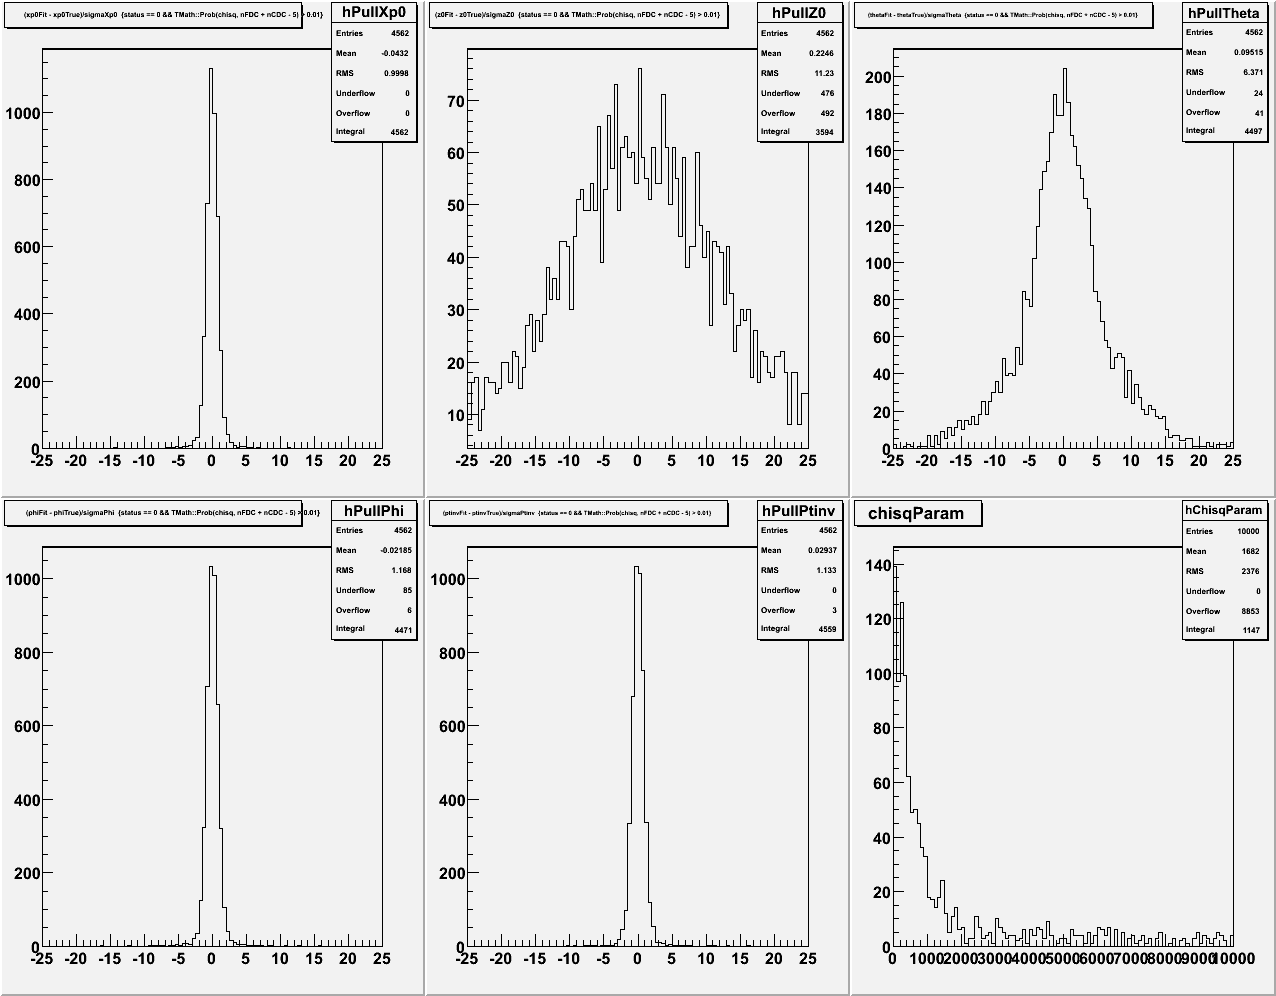
\includegraphics[height=3.0in]{pulls_guess.png}
$$
}

\f{
\ft{Pulls, True}
$$
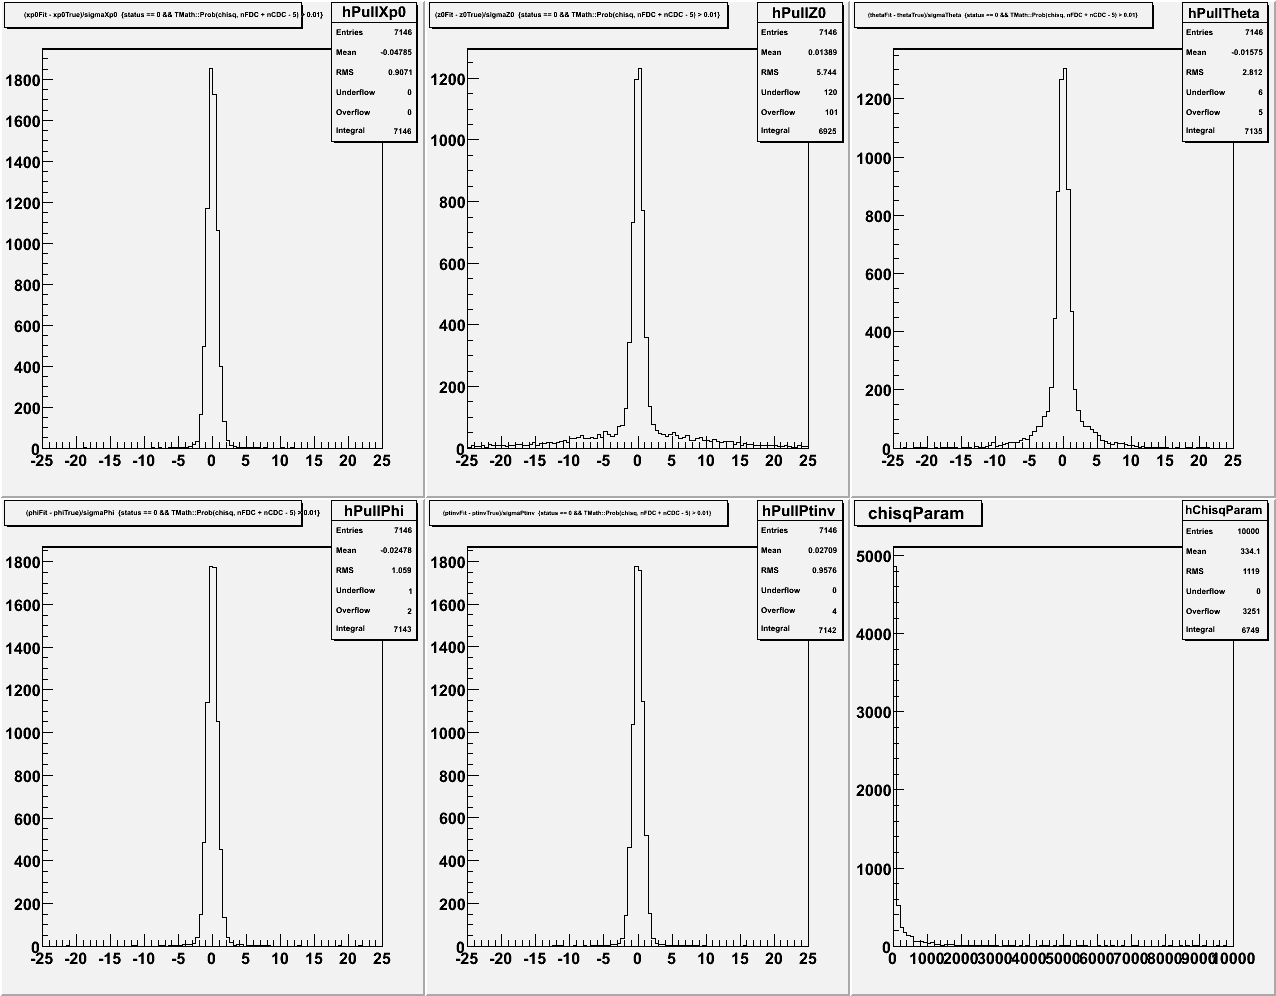
\includegraphics[height=3.0in]{pulls_true.png}
$$
}
\end{document}

%%% end of latex file %%%%
